\chapter{Production d'une source cohérente d'ondes de matière}
\label{ch:BEC_manip}
%\begin{tikzpicture}[remember picture, overlay]
%\node[anchor=north east,inner sep=0pt] at (current page.north east) {
\includegraphics[scale=1]{Fig/Chapter1/g825.png}};
%\end{tikzpicture}

Dans la partie précédente, nous nous sommes concentrés sur la physique que nous souhaitons étudier. En particulier, nous avons mis en évidence le fait que l'approche des atomes ultrafroids constitue une plateforme idéale pour l'étude de la propagation d'ondes dans un milieu désordonné, plateforme déjà éprouvée par l'observation de la localisation d'Anderson d'ondes de matières dans un désordre optique. 

À présent, concentrons-nous sur la description de l'un des deux éléments-clé de la propagation d'ondes dans le désordre: notre source d'ondes de matière. Le second élément, notre désordre optique, sera quant à lui présenté dans le chapitre \ref{ch:Speckle}.

Dans ce chapitre, nous nous attacherons donc à définir ce qu'est un condensat de Bose-Einstein puis nous décrirons ses principales propriétés. Dans un second temps, nous nous intéresserons aux outils dont nous disposons pour manipuler les atomes, puis nous terminerons en présentant la manière dont ces outils sont implémentés sur notre dispositif expérimental. 

\section{Condensation de Bose-Einstein}
Commençons par décrire ce qu'est un condensat de Bose-Einstein. Le phénomène de condensation a été prédit par Albert Einstein dans les années 1920 en s'appuyant sur les travaux de Satyendranath Bose traitant des statistiques quantiques pour des particules plus tard appelées \emph{bosons}. Il a cependant fallu attendre les années 1960 et le développement des premiers lasers pour voir émerger les premières techniques de manipulation d'atomes. La mise au point de telles technologies a d'ailleurs valu le prix Nobel à ses principaux architectes Claude Cohen-Tannoudji, Steven Chu et William D. Phillips en 1997. Enfin, le premier condensat de Bose-Einstein gazeux de ${}^{87}$Rb a été obtenu par l'équipe de Eric Cornell et Carl Wieman \citep{anderson1995observation}, rapidement suivi par un condensat de ${}^{23}$Na obtenu par Wolfgang Ketterle \citep{davis1995bose}. Ces travaux ont été récompensés par le prix Nobel de 2001.

\subsection{Statistique de Bose-Einstein}
Le phénomène de condensation de Bose-Einstein trouve son origine dans la statistique de Bose-Einstein. Celle-ci se différencie de la statistique classique de Boltzmann dans le formalisme grand-canonique donnée par:
\begin{equation}
N_{\mathbf{n}}=g_{\mathbf{n}} \exp{\left( -(E_{\mathbf{n}}-\mu)/k_{\mathrm{B}}T \right)}
\end{equation}
pour un gaz de $N$ particules à l'équilibre thermique, avec $N_{\mathbf{n}}$ le nombre moyen d'atomes présents dans l'état d'énergie $E_{\mathbf{n}}$ et de dégénérescence $g_{\mathbf{n}}$, $\mu$ le potentiel chimique, $T$ la température et $k_{\mathrm{B}}$ la constante de Boltzmann. L'origine de cette différence provient de l'indiscernabilité des particules: dans le cadre de la physique classique, les particules identiques sont discernables, c'est à dire qu'il est possible "d'étiqueter" les particules et de suivre leurs mouvements individuels.
Dans le cadre de la mécanique quantique, une telle approche n'est pas possible car les particules sont décrites par des fonctions d'onde, étalées dans l'espace. Lors de collisions de particules identiques, le recouvrement de leur fonction d'onde fait qu'il est impossible de déterminer les trajectoires suivies par les particules. L'indiscernabilité des particules dans le cadre de la mécanique quantique est donc essentielle.

\begin{figure}
\centering
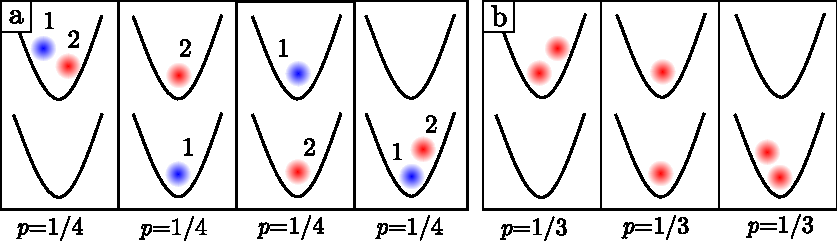
\includegraphics[width=\textwidth]{Fig/BEC_manip/stat_bose.pdf}
\caption{\textbf{a}: Répartition de deux particules discernables numérotées 1 et 2 sur deux niveaux d'énergie. Quatre configurations sont possibles. \textbf{b}: Répartition de deux particules indiscernables sur deux niveaux d'énergie. Dans le cas où ces particules peuvent se trouver dans le même état (bosons), trois configurations sont alors possibles.}
\label{fig:stat_bose}
\end{figure}

Considérons alors le cas simple de la répartition de deux particules sur deux niveaux d'énergie. Dans le cadre de la physique classique, il est possible d'attribuer un numéro à chaque particule, et il on peut placer chaque particule dans n'importe quel niveau d'énergie. Il existe alors quatre configurations que l'on supposera équiprobables, chacune de probabilité $p=1/4$ (voir figure \ref{fig:stat_bose}a). L'approche quantique, dans laquelle il n'est pas possible de discerner les particules, restreint le nombre de possibilités à trois et donc la probabilité de chacune des configurations est alors de $p=1/3$ (voir figure \ref{fig:stat_bose}b). Calculons maintenant la probabilité que deux particules soient dans le même état. En physique classique, cette probabilité est de $p=2/4=1/2$, tandis qu'en mécanique quantique, celle-ci est de $p=2/3$. On s'attend alors à ce que l'indiscernabilité des particules en mécanique quantique modifie la statistique de Boltzmann en favorisant l'agrégation de particules dans le même état \footnote{Ce raisonnement est valable pour des particules bosoniques, qui peuvent se retrouver dans le même état quantique. Pour des particules fermioniques, qui ne peuvent pas se retrouver dans le même état quantique, les statistiques en sont donc profondément changées. En guise d'illustration, la seule configuration possible de la figure \ref{fig:stat_bose}b pour des fermions est la seconde configuration.}.

\paragraph*{Condensation de Bose-Einstein}
Considérons alors le cas d'un gaz de $N$ bosons identiques dans un piège harmonique:
\begin{equation}
V(x,y,z)=\frac{1}{2}m \omega_x^2 x^2 + \frac{1}{2}m \omega_y^2 y^2 + \frac{1}{2}m \omega_z^2 z^2
\label{eq:piege_harmonique}
\end{equation}
où $m$ correspond à la masse des particules, et les $\omega_i$ correspondent aux fréquences de piégeage dans chaque direction de l'espace. Les énergies $E_{\mathbf{n}}$ sont donc celles des états liés
\begin{equation}
E_{\mathbf{n}}=\left(n_x+\frac{1}{2}\right) \hb \omega_x + \left(n_y+\frac{1}{2}\right) \hb \omega_y + \left(n_z+\frac{1}{2}\right) \hb \omega_z \quad \text{avec}\quad \mathbf{n}=\lbrace n_x,n_y,n_z\rbrace
\end{equation}

On peut alors montrer que le nombre moyen de particules est donné par la distribution de Bose-Einstein \footnote{Pour un gaz de $N$ fermions identiques, le nombre moyen de particules est donné par la distribution de Fermi-Dirac $ N_{\mathbf{n}}=\frac{g_{\mathbf{n}}}{\exp{\left( (E_{\mathbf{n}}-\mu)/k_{\mathrm{B}}T\right)}+1}$.}:\citep{diu1989elements}
\begin{equation}
N_{\mathbf{n}}=\frac{g_{\mathbf{n}}}{\exp{\left( (E_{\mathbf{n}}-\mu)/k_{\mathrm{B}}T \right)}-1}
\end{equation}
Une condition de validité de cette équation est que le potentiel chimique $\mu$ soit plus petit que l'énergie $E_{\mathbf{0}}$ du niveau de plus basse énergie, appelé niveau fondamental. Autrement, le nombre moyen de particules du niveau fondamental serait négatif (et cela impliquerait que la totalité du réservoir de particules vienne se déverser dans le niveau fondamental). Il est donc nécessaire que $\mu < E_0$. Une conséquence remarquable cette condition est que la population totale des états excités est bornée par:
\begin{equation}
N_e(\mu,T)=\sum_{\mathbf{n}\neq\mathbf{0}} N_{\mathbf{n}} \leq \sum_{\mathbf{n} \neq \mathbf{0}} \frac{g_{\mathbf{n}}}{\exp{\left( (E_{\mathbf{n}}-E_{\mathbf{0}})/k_{\mathrm{B}}T \right)}-1}
\end{equation}
Ainsi, chaque particule supplémentaire peuplera forcément l'état fondamental. On a donc ici le moyen d'accumuler un grand nombre de particules dans le même état quantique. La condensation de Bose-Einstein correspond, par définition, à cette accumulation d'un nombre macroscopique de particules dans l'état fondamental. Toutes ces particules peuplant cet état partagent alors le même état quantique. Afin d'atteindre un tel régime, il est nécessaire que les paquets d'onde des particules individuelles se recouvrent, c'est à dire que l'extension typique d'un paquet d'onde soit plus grande que la distance moyenne entre particules. L'extension typique de la fonction d'onde d'une particule peut être estimée à l'aide du principe d'incertitude de Heisenberg: $\Delta x \sim \hb / \Delta p$ avec $\Delta p \sim h/\lambda_{\mathrm{dB}}$. La grandeur $\lambda_{\mathrm{dB}}$ est homogène à une longueur et s'appelle la longueur d'onde thermique de de Broglie. Elle correspond à la taille typique d'un paquet d'onde quantique dont la largeur de la distribution en impulsion est donnée par la température. Celle-ci est donnée par \citep{diu1989elements}
\begin{equation}
\lambda_{\mathrm{dB}}=\sqrt{\frac{2\pi \hb^2}{m k_{\mathrm{B}}T}}
\end{equation}
avec m la masse de la particule, un atome de ${}^{87}$Rb dans le cas de notre expérience. La distance inter-particules dans un piège est estimée à partir de la densité de particules $d \sim n^{-1/3}$. On peut alors formuler le critère phénoménologique suivant:
\begin{equation}
n \lambda_{dB}^3 \gtrsim 1
\label{eq:critere_condensation}
\end{equation}
La quantité $n \lambda_{\mathrm{dB}}^3$ est appelée \emph{densité dans l'espace des phases}. Tout l'enjeu des expériences d'atomes ultrafroids est d'arriver à augmenter la densité dans l'espace des phases afin de franchir le seuil donné par l'équation \ref{eq:critere_condensation}. Cette condition peut se réécrire en terme de \emph{température critique}:
\begin{equation}
T_{\mathrm{C}}\sim \frac{\hb \overline{\omega}}{k_{\mathrm{B}}}N^{1/3}
\label{eq:temperature_critique}
\end{equation}
où $\overline{\omega}=(\omega_x \omega_y \omega_z)^{1/3}$ est la fréquence moyenne du piège. Cette température critique est de l'ordre de quelques centaines de nano-kelvin pour les expériences typiques d'atomes ultra-froids.


\subsection{Propriétés d'un condensat de Bose-Einstein}
En dessous de la température critique \ref{eq:temperature_critique}, les atomes s'accumulent dans l'état fondamental du piège. Il en résulte une forte augmentation de la densité, si bien qu'on ne peut plus négliger les interactions entre particules. Dans le cas d'un gaz suffisamment dilué, ce que l'on considèrera dans la suite, les interactions entre atomes peuvent être traitées comme des collisions à basse énergie, c'est à dire des collisions uniquement dans l'onde \emph{s}. Le potentiel d'interaction est alors celui de contact, donné par $U(\mathbf{r}_1-\mathbf{r}_2)=g\delta(\mathbf{r}_1-\mathbf{r}_2)$. Le paramètre $g$, qui caractérise la force des interactions, est donné par $g=\frac{4 \pi \hb^2}{m}a_{\mathrm{s}}$, avec $a_{\mathrm{s}}$ la longueur de diffusion, et ne dépend que de ce paramètre. Ce régime dilué est atteint lorsque $na_{\mathrm{s}}^3\ll 1$\footnote{Dans ce régime, la distance inter-atomique est plus grande que la portée des interactions. Ainsi, les atomes ne voient pas le détail du potentiel d'interaction avec leur voisin, et donc il est possible d'approximer ce potentiel par un potentiel de contact.}. Pour le ${}^{87}$Rb, cette longueur de diffusion vaut 100$a_{\mathrm{0}}>0$, avec $a_{\mathrm{0}}$ le rayon de Bohr. La longueur de diffusion étant positive, les interactions sont donc répulsives pour notre atome.

On peut écrire l'équation de Schrödinger pour l'état fondamental en tenant compte de ce terme d'interaction entre particules. La description en champ moyen du condensat est alors donnée par l'équation de Gross-Pitaevskii (aussi connue sous le nom d'\emph{équation de Schrödinger non-linéaire}):
\begin{equation}
i\hb \frac{\partial}{\partial t} \psi(\mathbf{r},t)=\left[-\frac{\hb^2}{2m}\Delta +V(\mathrm{r})+g\left| \psi(\mathbf{r},t) \right|^2 \right] \psi(\mathbf{r},t)
\label{eq:gross_pitaevskii}
\end{equation}
où $\psi(\mathbf{r},t)$ est la fonction d'onde macroscopique du condensat. La densité d'atomes est donnée par $n(\mathbf{r})= \left| \psi(\mathbf{r}) \right|^2$. Ainsi, la fonction d'onde du condensat $\psi(\mathbf{r},t)$ est normalisée pour donner le nombre de particules dans le condensat:
\begin{equation}
\int{\mathrm{d}\mathbf{r} \: \left| \psi(\mathbf{r},t) \right|^2}=N_{\mathbf{0}}
\end{equation}
Dans le régime stationnaire, on peut écrire $\psi(\mathbf{r},t)=\psi_0(\mathbf{r}) e^{i\mu t/\hb}$ avec $\mu$ le potentiel chimique du condensat, et l'injecter dans l'équation \ref{eq:gross_pitaevskii}. On obtient l'équation de Gross-Pitaevskii stationnaire:
\begin{equation}
\left[ -\frac{\hb^2}{2m}\Delta + V(\mathbf{r}) + g\left|\phi_0(\mathbf{r})\right|^2 \right] \phi_0((\mathbf{r}) = \mu \phi_0(\mathbf{r})
\end{equation}
Le premier terme de gauche décrit l'énergie cinétique, le second le terme d'énergie potentielle provenant du piège, et le dernier décrit l'énergie d'interaction entre particules, proportionnelle à la densité locale $n(\mathbf{r})=\left| \psi(\mathbf{r})\right|^2=\left| \phi_0(\mathbf{r}) \right|^2$. La somme de ces énergies donne le potentiel chimique $\mu$, qui correspond à l'énergie qu'il faut fournir pour rajouter une particule supplémentaire au système de $N$ particules.

\paragraph*{Régime de Thomas-Fermi}
Considérons le cas d'un condensat comportant un grand nombre de particules $N_0$. L'énergie cinétique totale du condensat varie avec $N_0$ de manière linéaire: $\mean{E_{\mathrm{k}}}\propto N_0$. L'énergie totale d'interaction varie quant à elle en $E_{\mathrm{int}}\propto N_0^2$. Pour un nombre suffisamment grand de particules, il devient possible de négliger le terme d'énergie cinétique dans l'équation de Gross-Pitaevskii stationnaire: il s'agit du régime de Thomas-Fermi.
Dans ce cas, le profil de densité s'écrit
\begin{equation}
n(\mathbf{r})=\left\{
					\begin{array}{ll}
						(\mu-V(\mathbf{r}))/g &\quad \text{lorsque} \quad \mu>V(\mathbf{r})\\
						0 &\quad \text{sinon}
					\end{array} 
				\right.
\end{equation}
et en considérant le piège harmonique de l'équation \ref{eq:piege_harmonique},
\begin{equation}
n(\mathbf{r})=\left\{
					\begin{array}{ll}
						\mu/g-\sum_{i=x,y,z}\frac{m\omega_i^2}{2g}r_i^2 &\quad \text{lorsque} \quad \mu>V(\mathbf{r})\\
						0 &\quad \text{sinon}
					\end{array} 
				\right.
\end{equation}
Le profil de densité est donc une parabole inversée de rayons
\begin{equation}
R_{\mathrm{TF},i}=\sqrt{\frac{2\mu}{m\omega_i^2}}
\end{equation}
Ces rayons de Thomas-Fermi ont été déterminés par la condition $n(\mathbf{r})=0$. Il est intéressant de noter que le potentiel effectif vu par une particule $V_{\mathrm{eff}}(\mathbf{r})=V(\mathbf{r})+gn(\mathbf{r})$ est constant sur l'ensemble du condensat:
\begin{equation}
V_{\mathrm{eff}}(\mathbf{r})= \left\{
									\begin{array}{ll}
										\mu &\quad \text{lorsque} \quad \mu>V(\mathbf{r})\\
										V(\mathbf{r}) &\quad \text{sinon}
									\end{array}
							\right.
\end{equation}
\begin{figure}
\centering
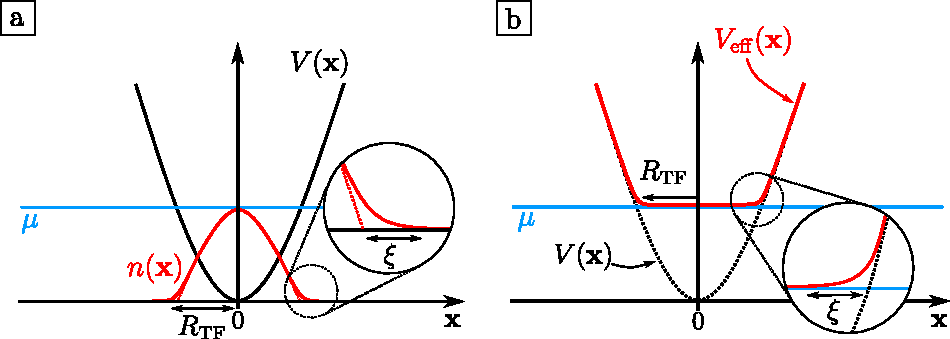
\includegraphics[width=\textwidth]{Fig/BEC_manip/thomas_fermi.pdf}
\caption{\textbf{a}: Profil de densité dans le régime de Thomas-Fermi. La densité est une parabole inversée, liée à la forme parabolique du potentiel. Sur les bords du condensat, la densité s'écarte de la parabole sur une longueur typique appelée longueur de cicatrisation. \textbf{b}: Potentiel effectif ressenti pour des particules individuelles. Ce potentiel effectif suit la forme du potentiel externe, et l'effet des interactions à l'intérieur du condensat écrante le potentiel externe par le potentiel chimique.}
\label{fig:thomas_fermi}
\end{figure}
Enfin, il est possible d'obtenir une expression pour le potentiel chimique \citep{pethick2008bose}: 
\begin{equation}
\mu=\frac{1}{2} \left( 15a N_{\mathbf{0}} \hb^2 \overline{\omega}^3 \right) ^{2/5} m^{1/5}
\end{equation}
et vaut environ $\mu/h\approx40$Hz pour notre expérience.

En réalité, l'approximation de Thomas-Fermi décrit bien les zones à l'intérieur des condensats, cependant, il existe une petite région sur les bords du condensat où la densité est faible, et donc l'énergie cinétique ne peut plus être négligée devant l'énergie d'interaction. Cette échelle de longueur s'appelle la longueur de cicatrisation, et est donnée par 
\begin{equation}
\xi=\sqrt{\frac{\hb^2}{n_{\mathbf{0}} mg}}
\end{equation}
avec $n_{\mathbf{0}}$ la densité moyenne du condensat. $\xi$ représente donc la longueur sur laquelle le potentiel chimique n'écrante pas le potentiel externe.


\section{Processus d'interaction lumière-matière}
Précédemment, nous avons brièvement présenté le phénomène de condensation de Bose-Einstein ainsi que les principales propriétés d'un condensat. En particulier, nous avons identifié un critère de condensation, qui sert de ligne à atteindre sur notre dispositif. À présent, nous allons présenter les différents outils de manipulation d'atomes dont nous disposons pour obtenir la condensation d'un nuage de rubidium ${}^{87}$Rb.
\subsection{Le rubidium ${}^{87}$Rb}
\label{sc:Rb87}
Comme déjà mentionné plusieurs fois, l'espèce atomique utilisée sur notre expérience est le rubidium ${}^{87}$Rb, le second isotope le plus abondant après le rubidium ${}^{85}$Rb (l'abondance naturelle du ${}^{87}$Rb est de 27.8\%). Il s'agit d'un alcalin (il possède donc un seul électron de valence) avec un spin nucléaire $\mathbf{I}=3/2$. Le choix de cet isotope repose sur l'existence d'une transition optique cyclante dans sa raie $D$. De plus, sa longueur de diffusion $a_{\mathrm{s}}=5.3$nm résulte en des taux de collisions relativement élevés, permettant une thermalisation rapide du nuage. À ce propos, il s'agit de l'atome ayant été condensé en premier. \citep{anderson1995observation}

La raie $D$ est en réalité composée de deux transitions: la raie $D_1$ correspondant à la transition $4^2S_{1/2}\rightarrow5^2P_{1/2}$ à 895nm, et la raie $D_2$ correspondant à la transition $5^2S_{1/2}\rightarrow5^2P_{3/2}$ à 780nm. Sauf mention contraire, nous n'utiliserons que la raie $D_2$ dans la suite de ce manuscrit, la plupart de nos fréquences optiques se trouvant à 780nm. La structure hyperfine de l'état fondamental $5^2S_{1/2}$ consiste en deux niveaux hyperfins dégénérés $\left| F=1 \right\rangle$ et $\left| F=2 \right\rangle$ séparés de $\Delta_{\mathrm{hf}}=6.835$GHz. Chacun de ces états est composé de $2F+1$ sous-états Zeeman. Une vue simplifiée de cette structure est donnée figure \ref{fig:Rb87}, et un tableau récapitulatif des principales grandeurs du ${}^{87}$Rb peut être trouvé table \ref{tbl:Rb87}.

\renewcommand{\arraystretch}{1.1}
\begin{table}[!ht]
\begin{center}
\begin{tabular}{ |c|c|c| }
\hline
\textbf{Quantité physique} & \textbf{Symbole} & \textbf{Valeur} \\
\hline
Masse & m & $1.44 \times 10^{-25}$kg \\
\hline
Fréquence de transition $D_2$ & $\omega_0$ & $2\pi \times 384.230$THz \\
\hline
Longueur d'onde dans le vide ($D_2$) & $\lambda_{\mathrm{0}}$ & 780.241nm \\
\hline
Largeur naturelle de la transition $D_2$ & $\Gamma$ & $2\pi \times 6.07$MHz \\
\hline
Fréquence de transition $D_1$ & $\omega_{D_1}$ & $2\pi \times 377.107$THz \\
\hline
Longueur d'onde dans le vide ($D_1$) & $\lambda_{D_1}$ & 794.979nm \\
\hline
Largeur naturelle de la transition $D_1$ & $\Gamma_{D_1}$ & $2\pi \times 5.75$MHz \\
\hline
Séparation hyperfine & $\Delta_{\mathrm{hf}}$ & 6.834682611GHz \\
\hline
Moment cinétique nucléaire & $\mathbf{I}$ & $3/2$ \\
\hline
Facteur de Landé électronique & $g_{\mathrm{S}}$ & 2.002319 \\
\hline
Facteur de Landé orbital & $g_{\mathrm{L}}$ & 0.999993\\
\hline
Facteur de Landé nucléaire & $g_{\mathrm{I}}$ & $-0.9951414 \times 10^{-3}$ \\
\hline
Intensité de saturation & $I_{\mathrm{sat}}$ & 1.67mW.cm${}^{-2}$ \\
\hline
Longueur de diffusion & $a_{\mathrm{s}}$ & 5.3nm \\
\hline
\end{tabular}
\end{center}
\caption{Tableau récapitulatif des grandeurs physiques du rubidium ${}^{87}$Rb que nous utiliserons dans la suite. Ces valeurs sont tirées de \citep{steck2001rubidium}.}
\label{tbl:Rb87}
\end{table}

\begin{figure}
\centering
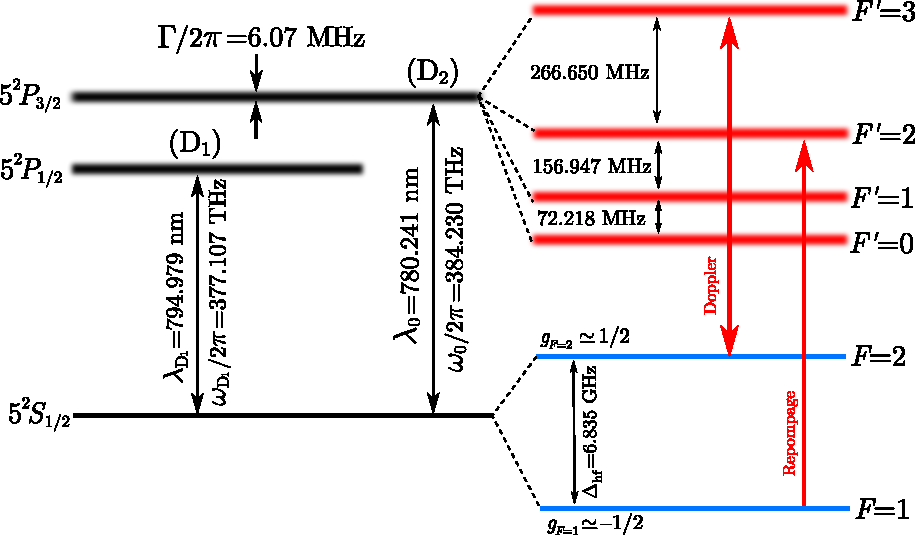
\includegraphics[width=0.8\textwidth]{Fig/BEC_manip/Rb87.pdf}
\caption{Structure de la raie $D$ du rubidium ${}^{87}$Rb. Celle-ci est composée de deux transitions, la $D_1$ à 795nm, et la transition $D_2$ à 780nm que nous utilisons sur l'expérience. L'état fondamental $5^2S_{1/2}$ est dégénéré en deux sous-niveaux hyperfins séparés d'une énergie $h \Delta_{\mathrm{hf}}$ avec $\Delta_{\mathrm{hf}}=6.835$GHz.}
\label{fig:Rb87}
\end{figure}

\subsection{Potentiel magnétique}
Commençons par décrire l'interaction d'un atome de rubidium avec un champ magnétique statique. Ces champs magnétiques sont couramment utilisés dans les expériences d'atomes ultra-froids pour réaliser des pièges conservatifs à l'aide champs inhomogènes (après un refroidissement laser par exemple). En particulier, l'expérience de Stern \& Gerlach montre que la force appliquée aux atomes par un gradient de champ magnétique dépend de l'état interne de l'atome. Explicitons cela.

Le moment cinétique total $\hat{\mathbf{F}}$ est donné par la somme des moments cinétiques des composants de l'atome:
\begin{equation}
\hat{\mathbf{F}}=\hat{\mathbf{I}}+\hat{\mathbf{L}}+\hat{\mathbf{S}}
\end{equation}
avec $\hat{\mathbf{I}}$ le spin total nucléaire, $\hat{\mathbf{L}}$ le moment cinétique orbital et $\hat{\mathbf{S}}$ le moment cinétique de spin électronique. On a alors un moment magnétique total $\hat{\boldsymbol\mu}=\mu_{\mathrm{B}} (g_{\mathrm{I}} \hat{\mathbf{I}} + g_{\mathrm{L}} \hat{\mathbf{L}} + g_{\mathrm{S}} \hat{\mathbf{S}})$ où les $g_{\mathrm{I},\mathrm{L},\mathrm{S}}$ sont les facteurs de Landé et $\mu_{\mathrm{B}}$ est le magnéton de Bohr. L'énergie d'interaction de ce moment magnétique avec un champ magnétique $\mathbf{B}$ est donnée par $\hat{V}=-\hat{\boldsymbol\mu}.\mathbf{B}$. On obtient les énergies propres par la formule de Breit-Rabi, dont l'application aux états $\left| F=1 \right\rangle$ et $\left| F=2 \right\rangle$ fournit:
\begin{equation}
\begin{aligned}
E_{F=2} &\simeq + \frac{h \Delta_{\mathrm{hf}}}{2} \sqrt{1+ m_F \beta +\beta^2} \\
E_{F=1} &\simeq - \frac{h \Delta_{\mathrm{hf}}}{2} \sqrt{1+ m_F \beta +\beta^2}
\end{aligned}
\end{equation}
avec $\beta \simeq 2 \mu_{\mathrm{B}} \left| B \right| /h \Delta_{\mathrm{hf}}$. À faible champ magnétique $\left| B \right| \ll h \Delta_{\mathrm{hf}} / \mu_{\mathrm{B}}$ (régime où $\beta \ll 1$), on retrouve l'effet Zeeman linéaire avec
\begin{equation}
U_{\mathrm{mag}}=m_{\mathrm{F}} g_{\mathrm{F}} \mu_{\mathrm{B}} \left| B \right|
\end{equation}
et $g_{\mathrm{F}=2}= 1/2$ et $g_{\mathrm{F}=1} =-1/2$. L'utilisation d'un champ magnétique non homogène génère donc un potentiel dépendant de la position, tel que dans l'expérience de Stern \& Gerlach. 
\begin{equation}
U_{\mathrm{mag}} (\mathbf{r}) = m_{\mathrm{F}} g_{\mathrm{F}} \mu_{\mathrm{B}} \left| B(\mathbf{r}) \right|
\end{equation}
L'utilisation de tels champs inhomogènes est très répandue dans le domaine des atomes ultra-froids, en particulier pour la génération de pièges magnétiques.







\subsection{Forces lumineuses}
\label{sc:forces_lumineuses}
On se concentre à présent sur l'interaction entre un atome et un champ laser incident. Ce champ laser comporte un grand nombre de photons émis par seconde (typiquement $10^{12}$ photons par seconde pour une puissance de 1µW), on peut donc décrire ce champ laser par une onde classique 
\begin{equation}
\mathbf{E}(\mathbf{r},t)= \mathrm{Re} \left( \underline{\mathbf{E}}(\mathbf{r}) e^{-i \omega t - i\phi (\mathbf{r})} \right)
\end{equation}
dont l'effet sur un atome est donné par le hamiltonien $H_{\mathrm{AL}}=-\mathbf{D}.\mathbf{E}(\mathbf{r},t)$. 
Dans la cadre de la théorie de la réponse linéaire, on introduit la polarisabilité atomique $\alpha(\omega)$ et on montre alors que la force moyenne exercée sur un atome est la somme de deux termes:
\begin{equation}
\mathbf{F}=\frac{1}{2} \mathrm{Re}(\alpha(\omega)) E(\mathbf{r}) \nabla E(\mathbf{r})+\frac{1}{2}\mathrm{Im}(\alpha(\omega)) E^2(\mathbf{r}) \nabla \phi(\mathbf{r})
\end{equation}

\paragraph*{Potentiel dipolaire}
Le premier terme est proportionnel à la partie réelle de la polarisabilité atomique. Ce terme décrit donc comment un moment dipolaire électrique induit interagit avec le gradient d'intensité lumineuse. On peut considérer cette force comme étant conservative et dérivant d'un potentiel qui est proportionnel à l'intensité lumineuse: on parle de \emph{potentiel dipolaire}. Dans le cas d'un faisceau très désaccordé, ce potentiel s'écrit:
\begin{equation}
U_{\mathrm{dip}}(\mathbf{r})=\frac{3\pi c^2 I(\mathbf{r})}{2 \omega_0^3} \left( \frac{\Gamma}{\omega - \omega_0} - \frac{\Gamma}{\omega + \omega_0} \right)
\end{equation}
avec $I(\mathbf{r})$ l'intensité lumineuse à la position $\mathbf{r}$. Cette expression est valable très loin de résonance: cela signifie que le laser ne voit pas le détail de la raie $D$ du ${}^{87}$Rb, c'est à dire que le désaccord $\omega-\omega_0$ doit être très grand devant la structure fine séparant les transitions $D_1$ et $D_2$. De plus, on a $\omega-\omega_0 \gg \Gamma$, avec $\Gamma$ la largeur de la transition.

Un tel potentiel présente de nombreux avantages pour les expériences d'atomes ultrafroids. Suivant le signe de la quantité $1/\overline{\Delta} = 1/(\omega-\omega_0)-1/(\omega+\omega_0)$, ce potentiel peut être soit attractif ($\overline{\Delta}<0$, on parlera alors de potentiel désaccordé vers le \emph{rouge}), soit répulsif ($\overline{\Delta}>0$, potentiel désaccordé vers le \emph{bleu}). Les atomes seront alors attirés par les maximas d'intensité lumineuse (pour un faisceau désaccordé vers le rouge) ou bien vers les zones d'ombre (pour les faisceaux désaccordés vers le bleu). Un faisceau gaussien focalisé désaccordé vers le rouge permet ainsi de piéger les atomes en son foyer: la forme gaussienne du faisceau attire les atomes vers le centre du faisceau. De plus dans cette limite, le potentiel est indépendant de l'état interne. Contrairement à un piège magnétique, un piège dipolaire n'est pas sélectif en état de spin et donc offre de nombreuses possibilités grâce à la disponibilité de degrés de liberté internes.

Cependant, l'utilisation de tels désaccords (plusieurs centaines de nano-mètres) contraint l'utilisation de grosses puissances optiques afin d'obtenir des potentiels suffisamment importants. Ainsi, il est courant que les expériences d'atomes ultrafroids utilisent des lasers de puissances de plusieurs Watts \footnote{À titre de comparaison, il ne suffit que de quelques milli-Watts pour endommager l'œil humain.} focalisés sur de petites tailles, typiquement quelques 10-100µm. Il se pose alors la question de la dissipation, liée à l'émission spontanée. Le taux d'émission spontanée peut être estimé par:
\begin{equation}
\Gamma_{\mathrm{sp}}(\mathbf{r})=\frac{3 \pi c^2 I(\mathbf{r})}{2\hb \omega_0^3} \left( \frac{\omega}{\omega_0}\right)^3 \left( \frac{\Gamma}{\omega-\omega_0}-\frac{\Gamma}{\omega+\omega_0} \right)^2
\end{equation}
et dans le cas dans d'un faisceau très désaccordé on peut souvent négliger ce taux et la dissipation qui lui est associée.

L'utilisation de désaccords plus modérés, typiquement de quelques nano-mètres, permet de fortement diminuer la puissance optique utilisée. En revanche, un tel rapprochement de la transition atomique implique qu'on ne peut plus négliger l'effet de la structure fine de la raie $D$. On peut alors considérer l'atome comme un système à non plus deux mais trois niveaux en négligeant la structure hyperfine de l'atome pour des désaccords gardés suffisamment grands $\omega-\omega_0 \gg \Delta_{\mathrm{hf}}$ et $\omega-\omega_{D_1} \gg \Delta_{\mathrm{hf}}$ (les séparations hyperfines des états excités sont plus petites que la séparation hyperfine des états fondamentaux).

Pour de tels désaccords et pour un faisceau polarisé linéairement, le potentiel dipolaire est alors donné par
\begin{equation}
U_{\mathrm{dip}}(\mathbf{r})=\frac{\pi c^2 I(\mathbf{r})}{2\omega_0^3} \left( \frac{\Gamma_{D_1}}{\omega-\omega_{D_1}} - \frac{\Gamma_{D_1}}{\omega+\omega_{D_1}} + \frac{2\Gamma}{\omega-\omega_0}-\frac{2\Gamma}{\omega+\omega_0}\right)
\end{equation}
Une conséquence de la structure fine est l'existence d'une zone entre les deux transitions où le potentiel est tantôt répulsif, tantôt attractif suivant que la fréquence du laser se rapproche de la fréquence de transition $D_1$ (répulsif) ou de la transition $D_2$ (attractif). Il existe donc une région dans laquelle il est possible de passer d'un potentiel désaccordé vers le bleu à un potentiel décalé vers le rouge sans croiser une transition atomique, comme illustré figure \ref{fig:v_dip_magique}. De plus, entre ces domaines de potentiel attractif et répulsif, il existe une longueur d'onde dite \emph{magique} pour laquelle le potentiel s'annule (les contributions des transitions $D_1$ et $D_2$ se compensent). Cette longueur d'onde est d'environ 790nm et peut être un véritable outil des expériences d'atomes ultrafroids, pour la réalisation d'un potentiel dépendant de l'état interne par exemple.

\begin{figure}
\centering
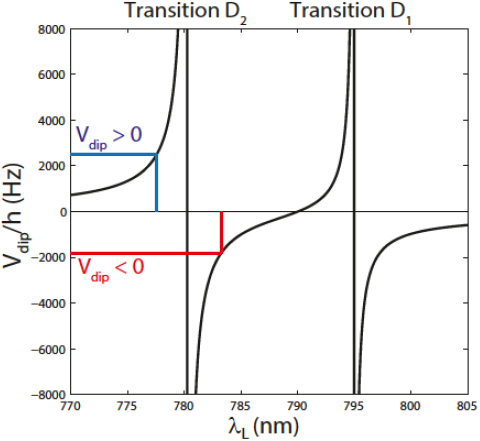
\includegraphics[scale=0.6]{Fig/BEC_manip/V_dip.png}
\caption{Potentiel dipolaire en fonction de la longueur d'onde du laser. La présence des deux transitions est remarquable par les deux divergences. Elles sont séparées par une zone de potentiel tantôt attractif, plus répulsif. Entre ces deux régimes se trouve une longueur d'onde \emph{magique} à environ 790nm pour laquelle le potentiel s'annule, quelque soit la puissance du laser.}
\label{fig:v_dip_magique}
\end{figure}

Naturellement, le rapprochement des transitions atomiques entraîne une augmentation du taux d'émission spontanée. Pour les désaccords considérés, il s'exprime
\begin{equation}
\Gamma_{\mathrm{sp}}=\frac{\pi c^2 I(\mathrm{r})}{2 \hb \omega_0^3} \left[ \left(\frac{\omega}{\omega_{D_1}} \right)^3 \left( \frac{\Gamma_{D_1}}{\omega-\omega_{D_1}} - \frac{\Gamma_{D_1}}{\omega+\omega_{D_1}} \right)^2 + 2\left( \frac{\omega}{\omega_0} \right)^3 \left( \frac{\Gamma}{\omega-\omega_0}-\frac{\Gamma}{\omega+\omega_0} \right)^2 \right]
\end{equation}
et l'ordre de grandeur du temps de vie associé est de l'ordre de quelques secondes.


Notons enfin qu'il est possible de se rapprocher encore plus de résonance et de devenir sensible à la structure hyperfine de la transition $D_2$ (dans ces conditions on peut négliger la contribution de la raie $D_1$). En revanche, le taux d'émission spontanée croît fortement et devient très contraignant.

\paragraph*{Force de pression de radiation}
Le second terme s'appelle \emph{force de pression de radiation}. Il provient de la partie imaginaire de la polarisabilité atomique, qui caractérise l'absorption de photons par l'atome. Il s'agit donc d'une force inélastique qui résulte d'un grand nombre de cycles d'absorption de photons du faisceau laser et d'émission spontanée dans des directions aléatoires de l'espace \footnote{Pour réaliser de tels cycles, il est nécessaire d'avoir une transition cyclante, c'est à dire de disposer d'un état excité dont la désexcitation renvoie forcément sur l'état d'origine}. L'impulsion totale cédée par émission spontanée s'annule donc, et en moyenne le transfert d'impulsion ne provient que de l'absorption de photons du faisceau laser. Cette force est donnée par
\begin{equation}
\mathbf{F}_{\mathrm{PR}}=\hb \mathbf{k} \Gamma_{\mathrm{sp}} 
\end{equation}
avec $\Gamma_{\mathrm{sp}}$ le taux d'émission spontanée en présence du champ laser, et $\mathbf{k}$ le vecteur d'onde associé à l'onde laser. L'interprétation est directe: en moyenne, l'atome acquiert une impulsion $\hb \mathbf{k}$ à un taux $\Gamma_{\mathrm{sp}}$. Ce taux vaut:
\begin{equation}
\Gamma_{\mathrm{sp}}=\frac{\Gamma}{2} \frac{s}{1+s}
\end{equation}
et $s$ s'appelle le paramètre de saturation. Celui-ci dépend de l'intensité lumineuse incidente (et donc du nombre de photons incidents) ainsi que du désaccord du laser par rapport à la résonance atomique $\delta = \omega-\omega_0$. Il s'exprime
\begin{equation}
s=\frac{I/I_{\mathrm{sat}}}{1+4\delta^2/\Gamma^2}
\end{equation}
où l'intensité de saturation $I_{\mathrm{sat}}=\frac{\pi h c \Gamma}{3\lambda_0^3}=1.67$mW.cm${}^{-2}$ est une constante de l'atome de ${}^{87}$Rb. Le paramètre de saturation est maximal en $\delta=0$, c'est à dire lorsque le laser est à résonance. Dans le cas d'un laser très saturant $s \gg 1$, la force de pression de radiation s'écrit
\begin{equation}
\mathbf{F}_{\mathrm{PR}}=\frac{\hb \mathbf{k} \Gamma}{2}
\end{equation}
où le facteur 2 indique que à forte saturation, un atome autant de chance d'être dans l'état excité que dans l'état fondamental. Enfin, mentionnons que pour un atome se déplaçant à une vitesse $\mathbf{v}$ dans le référentiel du laboratoire, le désaccord devient $\delta=\omega-\omega_0-\mathbf{k}.\mathbf{v}$ par effet Doppler.


\subsection{Couplage radio-fréquence} 
Les outils de manipulation des atomes présentés précédemment offrent la possibilité de créer des potentiels conservatifs (comme le potentiel dipolaire ou le potentiel magnétique) ou encore des forces dissipatives à l'aide la force de pression de radiation. Néanmoins, la plupart d'entre elles dépend de l'état interne de l'atome. Un bon contrôle de cet état interne permet non seulement d'assurer une bonne répétabilité de l'expérience, mais aussi de proposer des solutions technologiques originales. 

Comme présenté section \ref{sc:Rb87}, la séparation entre les états fondamentaux $\left| F=1 \right\rangle$ et $\left| F=2 \right\rangle$ correspond à une fréquence $\Delta_{\mathrm{hf}}$ de l'ordre du GHz, donc à une fréquence qui se trouve accessible électroniquement. De plus, ces états étant fondamentaux, ils ne peuvent pas se désexciter. Un couplage radio-fréquence entre ces états apparaît alors comme un formidable outil de contrôle de l'état interne des atomes.

Dans ces conditions, les états fondamentaux hyperfins du ${}^{87}$Rb s'avèrent réaliser une excellente approximation d'un système à deux niveaux dont le hamiltonien propre est donné dans la base $\left\lbrace \left|F=1\right\rangle, \left|F=2\right\rangle \right\rbrace$ par
\begin{equation}
\hat{H}_0=\frac{\hb}{2} \begin{pmatrix}
-\Delta_{\mathrm{hf}} & 0 \\
0 & \Delta_{\mathrm{hf}}
\end{pmatrix}
\end{equation}
Le couplage par radio-fréquences est quant à lui décrit par le hamiltonien
\begin{equation}
\hat{V}(t)=\frac{\hb}{2} \begin{pmatrix}
0 & \Omega e^{i \omega t} \\
\Omega e^{-i\omega t} & 0
\end{pmatrix}
\label{eq:couplage_rabi}
\end{equation}
avec $\omega$ la fréquence de l'onde radio-fréquence rayonnée sur les atomes, et $\Omega$ la pulsation de Rabi qui caractérise l'amplitude rayonnée sur les atomes. Le terme de couplage \ref{eq:couplage_rabi} est obtenu en appliquant l'approximation de l'onde tournante, c'est à dire que l'on néglige les termes en $\omega +\Delta_{\mathrm{hf}}$ devant les termes en $\omega - \Delta_{\mathrm{hf}}$ car on estime qu'ils évoluent rapidement, et donc qu'ils s'apparentent à leur valeur moyenne qui est nulle. En se plaçant dans le référentiel tournant, le hamiltonien $\hat{H}_0+\hat{V}$ du système devient
\begin{equation}
\hat{H}=\frac{\hb}{2} \begin{pmatrix}
\delta & \Omega \\
\Omega & -\delta
\end{pmatrix}
\end{equation}
avec $\delta=\omega- \Delta_{\mathrm{hf}}$. En supposant que le système est dans l'état $\left| F=1 \right\rangle$ à $t=0$, la probabilité d'avoir l'atome dans l'état $\left| F=2 \right\rangle$ est donnée par la formule de Rabi \citep{basdevant2002mecanique}
\begin{equation}
\mathcal{P}_{\left| F=2 \right\rangle}(t)= \frac{\Omega^2}{\Omega^2+\delta^2} \sin^2{\left(\sqrt{\Omega^2+\delta^2} \frac{t}{2} \right) }
\label{eq:rabi_formule}
\end{equation}
Cette formule met en évidence un caractère résonant des transitions radio-fréquences:
\begin{itemize}
\item[\textendash] Dans le cas d'un grand désaccord $\delta \gg \Omega$, la probabilité de transition est très faible à n'importe quel instant.
\item[\textendash] À résonance $\delta=0$, la probabilité de transition peut atteindre 1, même si l'amplitude de l'onde rayonnée est très faible ($\Omega$ petit).
\end{itemize}
Ces caractéristiques peuvent être retrouvées figure \ref{fig:rabi}. En effet, l'enveloppe lorentzienne représentée figure \ref{fig:rabi}b montre les populations maximales transférées, faibles lorsque $\| \delta \| > \Omega$. On retrouve la condition de résonance à $\delta=0$, et le transfert est maximal lorsque la durée d'application du champ radio-fréquence $t_p$ satisfait
\begin{equation}
t_p=(2n+1) \frac{\pi}{\Omega}
\end{equation}

\begin{figure}
\centering
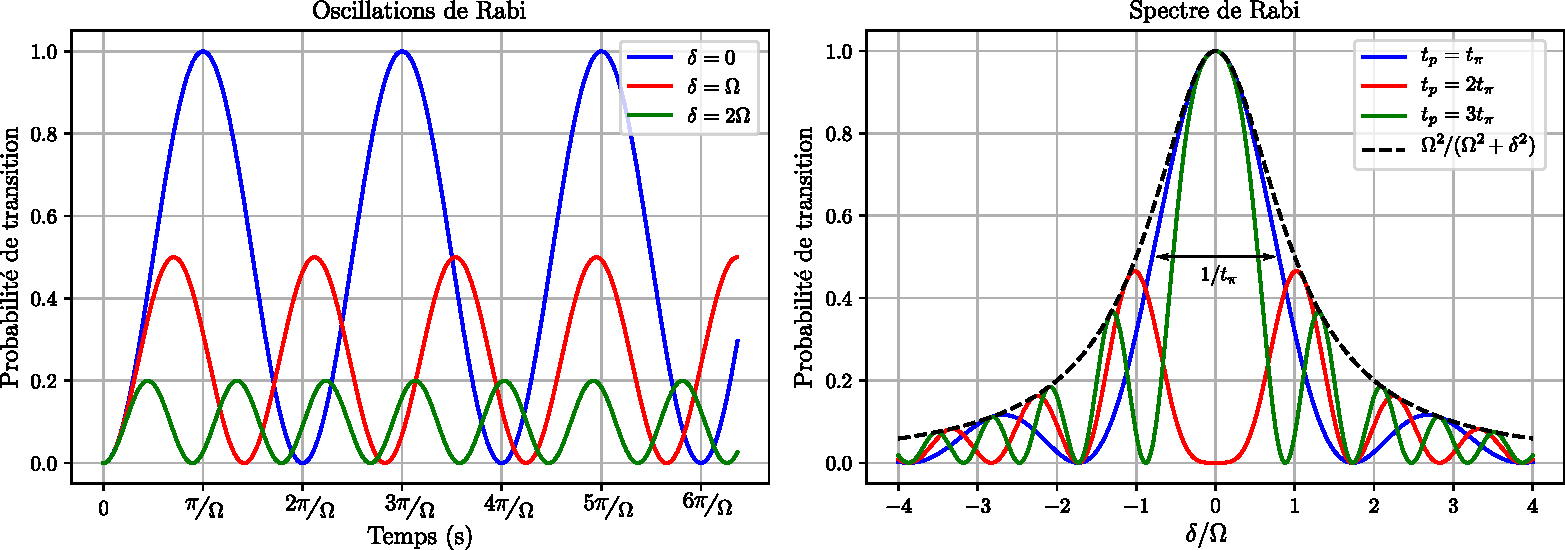
\includegraphics[width=\textwidth]{fig/BEC_manip/rabi.pdf}
\caption{\textbf{a}: Oscillations de Rabi tracées pour différents désaccords. Les populations oscillent à la fréquence $\sqrt{\Omega^2+\delta^2}$ avec une amplitude qui dépend du désaccord. L'amplitude est maximale et atteint 1 lorsque l'onde radio-fréquence est à résonance, et la population maximale transférée décroît avec l'augmentation du désaccord. \textbf{b}: Spectres de Rabi pour différentes durées d'application $t_p$. Le transfert de population est le plus efficace à résonance ($\delta=0$) pour certaines durées telles que $t_p= (2n+1) \pi/ \Omega$. On retrouve bien l'enveloppe lorentzienne de l'équation \ref{eq:rabi_formule}.}
\label{fig:rabi}
\end{figure}






\section{Description d'un cycle expérimental}
Dans la partie précédente, nous nous sommes familiarisés avec quelques outils couramment utilisés sur les expériences d'atomes ultrafroids pour piéger et manipuler les atomes. Dans cette nouvelle partie, nous nous pencherons sur l'implémentation de ces outils sur notre expérience afin d'obtenir un condensat de Bose-Einstein de ${}^{87}$Rb. La présentation qui en sera donnée ici se verra succincte, nous nous contenterons d'illustrer brièvement les différentes étapes de refroidissement qui mènent à la condensation. De nombreux détails pourront être trouvés dans les thèses des doctorants qui ont contribué à faire de cette expérience ce qu'elle est aujourd'hui: \citep{fauquembergue2004realisation}, \citep{riou2006etude}, \citep{bernard2010transport}, \citep{jendrzejewski2012quantum}, \citep{muller2015coherent}, \citep{denechaud2018vers}... 

\subsection{Présentation générale du dispositif}
Comme toutes les expériences d'atomes ultra-froids, la manipulation des atomes se déroule sous ultra-vide afin de s'affranchir des conditions extérieures. En particulier, on évite ainsi les collisions avec des particules extérieures à température ambiante, ce qui chaufferait notre gaz et détruirait la cohérence d'un nuage condensé. Une vue d'ensemble de l'enceinte à vide est donnée figure \ref{fig:manip} qui montre aussi les pompes utilisées en continu pour maintenir le vide. Notre dispositif est composé d'un four chauffé à 120°C qui éjecte les atomes de rubidium, il s'agit de notre source d'atomes. Un doigt froid refroidi à -30°C sert de diaphragme et permet de filtrer le jet d'atomes tout en adsorbant les atomes qui sont bloqués afin de pas polluer le vide. Un obturateur mécanique permet de couper le jet lorsqu'on ne souhaite pas accumuler des atomes en cours de cycle. Les atomes sont décélérés dans le ralentisseur Zeeman et capturés dans la première cellule où ils subissent les premières étapes de refroidissement. Ils sont ensuite transportés dans la seconde cellule où ils sont refroidis jusqu'à la condensation. C'est dans cette seconde cellule que se déroulent les expériences de science, on l'appelle alors \emph{Chambre de science}.

\begin{figure}
\centering
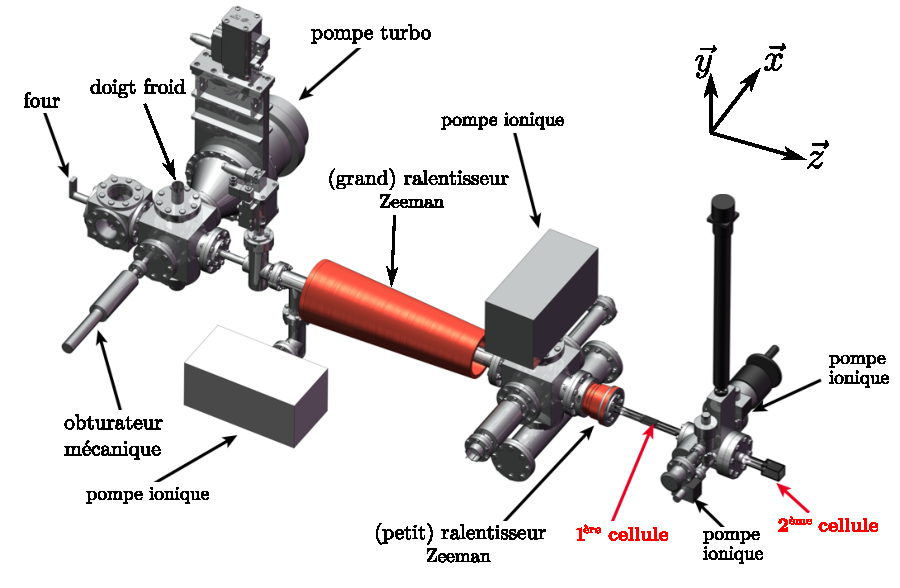
\includegraphics[width=\textwidth]{Fig/BEC_manip/manip.pdf}
\caption{\textbf{Vue d'ensemble du corps de l'expérience.} Les atomes se trouvent dans un montage sous ultra-vide, composé de deux chambres dans lesquelles les atomes sont manipulés.}
\label{fig:manip}
\end{figure}

\subsection{Première chambre}
C'est dans la première chambre que se déroulent les premières étapes de refroidissement du gaz de rubidium. Celles-ci sont dans un premier temps basées sur le refroidissement laser, puis dans un second temps sur un piégeage magnétique et l'évaporation forcée à l'aide d'un couteau radio-fréquence.

\paragraph*{Refoidrissement laser}
Le principe du refroidissement laser repose sur la force de pression de radiation, présentée section \ref{sc:forces_lumineuses}. Une compréhension du phénomène de refroidissement laser peut être donnée à l'aide du désaccord $\delta=\omega-\omega_0- \mathbf{k}. \mathbf{v}$ dans le cas d'un atome se déplaçant à vitesse $\mathbf{v}$.
Dans le référentiel de l'atome, la condition de résonance $\delta=0$ s'écrit $\omega_0=\omega-\mathbf{k}.\mathbf{v}$. L'atome va donc absorber un photon d'énergie $\hb \omega$ et en émettre un d'énergie $\hb \omega_0$ (d'énergie plus grande que le photon absorbé dans la cas d'un décalage vers le rouge par effet Doppler). Il y a donc eu un transfert d'énergie entre l'énergie cinétique et le désaccord. La répétition de tels cycles permet ainsi de transférer beaucoup d'énergie cinétique de l'atome vers le désaccord entre photons absorbés et photons rayonnés.

La possibilité de répéter ces cycles d'absorption de photons et d'émission spontanée repose sur l'existence d'une transition cyclante entre les états hyperfins $\left| F=2 \right\rangle$ et $\left| F'=3 \right\rangle$. La désexcitation de $\left|F'=3\right\rangle$ renvoie forcément l'atome dans l'état $\left| F=2 \right\rangle$ car les règles de sélection imposent $F'-F= \lbrace 0, \pm 1 \rbrace$.
En revanche, on peut accidentellement envoyer des atomes dans l'état excité $\left| F'=2 \right\rangle$ car la séparation avec l'état ciblé $\left| F'=3 \right\rangle$ n'est que de 266MHz. Statistiquement, un atome visite cet état tous les 50 cycles environ, et sa désexcitation peut faire tomber les atomes dans l'état $\left|F=1\right\rangle$. Cet état étant un état noir, pour conserver les atomes, on doit alors utiliser un second laser appelé \emph{repompeur} qui permet de recycler les atomes perdus vers la transition cyclante\footnote{À titre d'illustration, le temps de vie du piège magnéto-optique a été mesuré à une dizaine de secondes. Sans le faisceau repompeur, les atomes tombent dans l'état noir $\left| F=1 \right\rangle$ en quelques micro-secondes seulement.}. Il est accordé sur la transition $\left| F=1 \right\rangle \rightarrow \left| F'=2 \right\rangle$.

Notre dispositif laser se compose alors d'un laser principal de refroidissement accordé sur la transition $\left| F=2 \right\rangle \rightarrow \left| F'=3 \right\rangle$. Il est secondé d'un second laser \emph{repompeur} accordé sur la transition $\left| F=1 \right\rangle \rightarrow \left| F'=2 \right\rangle$. Enfin un dernier laser sert de référence de fréquence pour les deux précédents en étant asservi par absorption saturée. Une représentation schématique de l'ensemble de ces lasers et de leur amplification peut être trouvée figure \ref{fig:table_optique}.

\begin{figure}
\centering
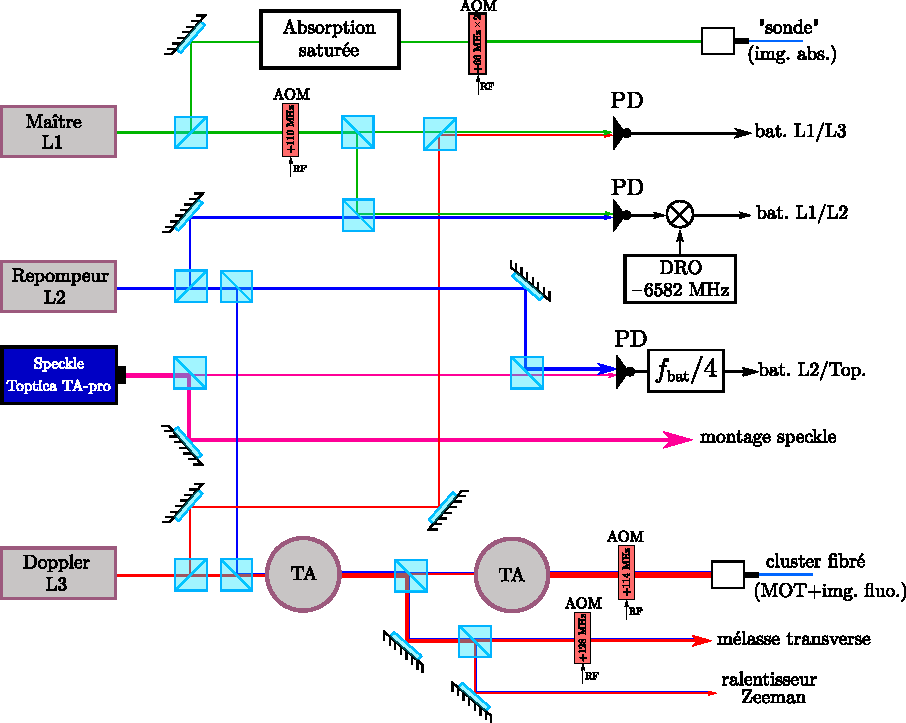
\includegraphics[width=0.8\textwidth]{Fig/BEC_manip/table_optique.pdf}
\caption{\textbf{Représentation schématique de notre montage laser.} Le laser maître \emph{L1} sert de référence de fréquence en étant asservi par absorption saturée. Le laser de refroidissement Doppler \emph{L3} est asservi par battements avec \emph{L1}. Le laser repompeur \emph{L2} est lui aussi asservi par battements avec L2 grâce à l'utilisation d'électronique rapide. Notons enfin que les faisceaux de \emph{L2} et \emph{L3} sont mélangés avant amplification (TA). Les faisceaux arrivant sur les atomes comporteront alors les fréquences provenant de ces deux lasers. Un obturateur mécanique (non représenté) permet de couper le faisceau de \emph{L2} allant vers les amplificateurs. {\LARGE POMPAGE OPTIQUE}}
\label{fig:table_optique}
\end{figure}

\paragraph*{Le ralentisseur Zeeman}
La première étape consiste à ralentir suffisamment le jet d'atomes pour pouvoir les capturer dans un premier piège. Un laser désaccordé vers le rouge par rapport à la transition cyclante $\left| F=2 \right\rangle \rightarrow\left| F'=3 \right\rangle$ permet de réaliser une décélération des atomes à l'aide de cycles d'absorption et d'émission spontanée de photons. Cependant, le ralentissement des atomes entraîne un eloignement de la résonance à cause de l'effet Doppler. Pour palier à ce problème, on applique un champ magnétique pour satisfaire localement la condition de résonance par effet Zeeman. Ce champ est appliqué à l'aide d'une bobine comportant un nombre de tours par unité de longueur variable, représentée figure \ref{fig:manip} entre le four et la première chambre.
Ainsi, on est capable de réduire la vitesse des atomes de 100m.s${}^{-1}$ à environ 20m.s${}^{-1}$ sur une distance de seulement 1m.

\paragraph*{Le piège magnéto-optique}
Une fois les atomes suffisamment ralentis, ils sont capturés dans le piège magnéto-optique (abrégé en \emph{MOT} pour l'anglais \textit{Magneto-Optical Trap}). Celui-ci est composé de trois paires de faisceaux contra-propageants désaccordés vers le rouge d'environ $\delta=-16$MHz, de polarisations opposées $\sigma^+$ et $\sigma^-$. Chacun de ces faisceaux possède une puissance d'environ 12mW.
De plus, deux bobines en configuration anti-Helmholtz permettent de générer un champ quadrupolaire, donc un gradient magnétique dans les trois directions de l'espace, afin de créer une force de rappel.
On charge environ $2 \times 10^9$ atomes en moins d'une seconde grâce à la mélasse transverse qui permet de collimater le jet d'atomes et donc d'améliorer le flux. 
Une fois le chargement saturé, on coupe le champ magnétique pendant quelques millisecondes afin de réduite fortement la température: c'est l'étape de mélasse optique qui permet de descendre la température à environ 50µK. 

\begin{figure}
\centering
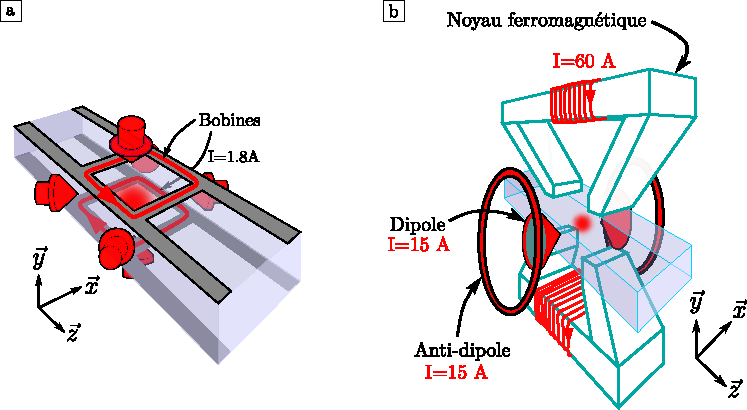
\includegraphics[width=\textwidth]{Fig/BEC_manip/MOT_magtrap.pdf}
\caption{\textbf{a: Éléments du piège magnéto-optique.} Il est réalisé à l'aide de trois paires de faisceaux contra-propageants et de deux bobines formant un champ quadrupolaire. Ces bobines sont faites à partir de circuits imprimés posés sur la cellule. \textbf{b: Géométrie du piège magnétique.} Un champ quadrupolaire intense est créé selon les directions $\vec{y}$ et $\vec{z}$ par un électroaimant. Un champ de biais est généré par deux paires de bobines suivant la direction $\vec{x}$. Ce champ possède une courbure longitudinale et est responsable du confinement suivant cette direction. }
\label{fig:MOT_magtrap}
\end{figure}

\paragraph*{Piège magnétique et évaporation radio-fréquence}
Après l'étape de mélasse, on souhaite manipuler les atomes dans un piège magnétique. Afin d'augmenter le nombre d'atomes piégeables magnétiquement, il est nécessaire de manipuler l'état interne des atomes. On procède ainsi à une étape de dépompage en éteigant le faisceau de repompage et en accordant le faisceau de refroidissement sur la transition $\left| F=2 \right\rangle \rightarrow\left| F'=2 \right\rangle$: en moins d'une milliseconde, les atomes se trouvent dans l'état $\left| F=1 \right\rangle$, dont seul le sous-état zeeman $\left| F=1, m_{\mathrm{F}}=-1 \right\rangle$ peut être piégé\footnote{Il est le seul des trois sous-états zeeman de $\left| F=1 \right\rangle$ à avoir le produit $g_{\mathrm{F}} m_{\mathrm{F}} > 0$, c'est à dire qu'il s'agit d'un état \emph{Low Field Seeker}, qui est attiré par les zones de faible champ magnétique. En effet, c'est à l'aide d'un minimum de champ magnétique que l'on réalise ce piège, le théorème de Wing interdisant les maximas de champ magnétique. }\footnote{Des huit sous-états zeeman fondamentaux, il s'agit de celui ayant la plus grande probabilité d'occupation tout en étant piégeable, justifiant son choix. }. Afin de maximiser la population de ce sous-état, on allume un faisceau de pompage optique accordé sur la transition $\left| F=1 \right\rangle \rightarrow \left| F'=1 \right\rangle$ et polarisé $\sigma^-$ pendant 40µs. En parallèle, on allume le champ du dipôle afin de définir un axe de quantification.

Le piège magnétique que l'on utilise est un piège de type \emph{Ioffe-Pritchard}. Il est composé essentiellement de deux éléments:
\begin{itemize}
\item[\textendash] Un champ de biais orienté dans la direction $\vec{x}$, généré par une paire de bobines (\emph{dipôle}) de configuration légèrement plus éloignée que celle de Helmholtz: on a ainsi une courbure positive dans la direction longitudinale au centre des bobines. Une seconde paire de bobines (\emph{anti-dipôle}) permet d'abaisser le champ constant au centre du piège, et donc de le comprimer \citep{fauquembergue2004realisation}.
\item[\textendash] Un champ quadrupolaire dans le plan $(\vec{y},\vec{z})$ généré par un électroaimant ferromagnétique épais (\emph{quadrupôle}) comportant deux entrefers et deux bobines excitatrices dans deux sens opposés. L'épaisseur importante du matériau magnétique minimise l'effet de l'électroaimant dans la direction $\vec{x}$.
\end{itemize}
Le confinement dans la direction $\vec{x}$ est donc réalisée par le champ de \emph{dipôle}, tandis que le confinement dans les directions $\vec{y}$ et $\vec{z}$ est fait par le \emph{quadrupôle}. 
La présence du champ de dipôle permet aussi de s'affranchir des pertes par transition Majorana, le champ ne s'annulant à aucun endroit de l'espace.
On obtient ainsi un nuage piégé magnétiquement comportant environ $1 \times 10^9$ atomes tous dans le même sous-état zeeman à une température de $\sim 300$ µK.

Une fois le nuage thermalisé, on procède à une étape de refroidissement évaporatif grâce à la méthode de \emph{couteau radio-fréquence}. Le principe du refroidissement évaporatif sera détaillé section \ref{sc:evap_optique}, mais on peut le résumer de la manière suivante:
\begin{itemize}
\item[\textendash]On tronque le piège de telle sorte que quelques atomes très énergétiques (la queue de la distribution de vitesses de Maxwell-Boltzmann) puisse s'échapper du piège.
\item[\textendash]Les collisions entre les particules étant restées dans le piège permettent au système de retourner à l'équilibre thermique à une température plus basse.
\end{itemize}
La troncature du piège se fait à l'aide d'une onde radio-fréquence rayonnée par les bobines MOT. Celle-ci induit une transition de l'état piégé $\left| F=1, m_{\mathrm{F}}=-1 \right\rangle$ à l'état non piégé $\left| F=1, m_{\mathrm{F}}=0 \right\rangle$ lorsque la condition de résonance $\hb \omega_{\mathrm{RF}} = m_{\mathrm{F}} g_{\mathrm{F}} \mu_{\mathrm{B}} B(\mathbf{r})$ est vérifée. En abaissant progressivement la fréquence rayonnée pendant une dizaine de secondes, on obtient finalement un nuage de $70 \times 10^6$ atomes à une température de 10µK.

\begin{figure}
\centering
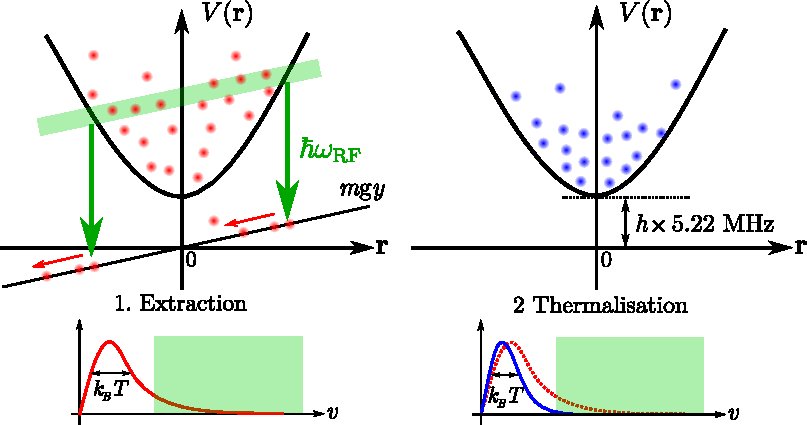
\includegraphics[width=0.9\textwidth]{Fig/BEC_manip/evapRF.pdf}
\caption{\textbf{Principe de l'évaporation radio-fréquence.} L'application d'une radio-fréquence permet de tronquer le piège magnétique, et d'éliminer les atomes les plus énergétiques. L'énergie moyenne par particule étant plus basse, la température s'en retrouve abaissée après thermalisation.}
\label{fig:evapRF}
\end{figure}


\subsection{Chambre de science}
Présentation du transport, du piège croisé, de la lévitation, spin-flips. Delta-kick

Après ces premières étapes de refroidissement, les atomes sont transportés dans une seconde cellule où l'on procède à une évaporation tout-optique pour franchir le seuil de condensation. La raison d'être de cette seconde cellule est de profiter d'un maximum d'accès optiques tout en s'affranchissant de l'environnement magnétique de la première chambre, en particulier celui du ferromagnétique.
Nous nous contenterons ici de présenter les grandes lignes des éléments de cette seconde chambre, de nombreux détails pourront être trouvés dans la thèse d'Alain Bernard \citep{bernard2010transport}, dans la thèse de Fred Jendrzejewski \citep{jendrzejewski2012quantum} et de Kilian Muller \citep{muller2015coherent}. De plus, certains de ces éléments ont été modifiés au cours de ma thèse et une étude plus approfondie en sera présentée dans le chapitre \ref{ch:new_exp}.

\paragraph*{Transport dans une pince optique et piège dipolaire croisé}
Après évaporation radio-fréquence, on transfert le nuage dans une pince optique. Il s'agit d'un piège dipolaire créé par focalisation sur les atomes d'un faisceau laser de longueur d'onde $\lambda=$1070nm et de puissance estimée d'environ 1.5W. Dans le plan focal, ce faisceau a une taille $\mathrm{w}_{\mathrm{0}}=$28µm et la distance de Rayleigh vaut donc $z_{\mathrm{R}}= \pi \mathrm{w}_{\mathrm{0}}^2 / \lambda$ = 2.3mm. On obtient ainsi $10 \times 10^6$ atomes à une température de 10µK aux alentours du foyer de la pince\footnote{Ce faible taux de transfert entre le piège magnétique et la pince porvient du mauvais recouvrement spatial entre ces deux pièges. La pince est très alongée suivant la direction $\vec{z}$, tandis que le piège magnétique est étendu suivant la direction $\vec{x}$. Cette géométrie est un héritage des débuts de cette expérience, originellement utlisée pour étudier le laser à atomes.}.

Le transport dans la seconde chambre se fait à l'aide d'une platine de translation montée sur coussin d'air \emph{Aerotech ABL80040}. Les optiques de focalisation de la pince se trouvant sur cette platine, on déplace ainsi les atomes de 40cm en moins de 2s, comme illustré figure \ref{fig:piege_optique}. On estime l'efficacité de transfert à 75\%, mesurée en effectuant un aller-retour pour retourner dans la première chambre.

\begin{figure}
\centering
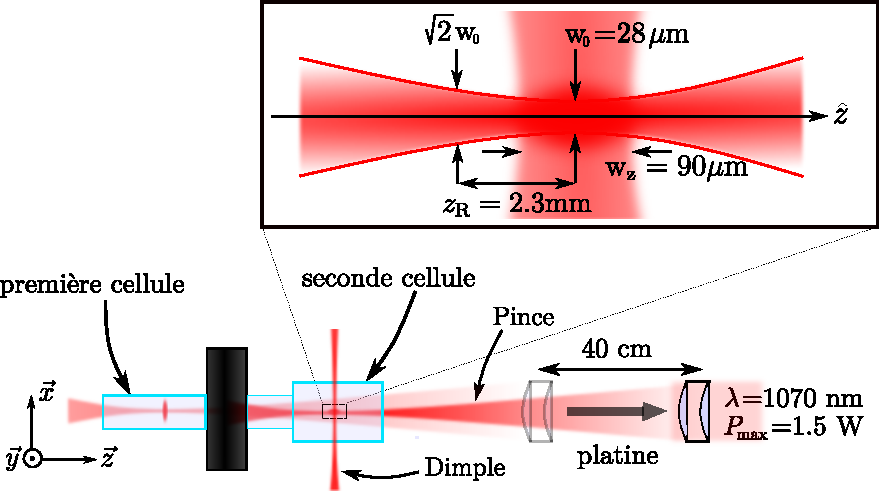
\includegraphics[width=0.9\textwidth]{Fig/BEC_manip/piege_optique.pdf}
\caption{\textbf{Illustration du transport et du piège optique.} Les atomes sont capturés autour du foyer de la pince dans la première chambre, et le point de focalisation est déplacé de 40cm à l'aide d'une platine de translation. Une fois le transport terminé, on allume un second faisceau de piegeage vertical (\emph{dimple}).}
\label{fig:piege_optique}
\end{figure}

Une fois les atomes arrivés dans la seconde chambre, un second faisceau de piégeage dipolaire de longueur d'onde 1070nm et de puissance 7W est allumé afin de comprimer le nuage suivant la direction $\vec{z}$ qui correspond à la direction longitudinale de la pince. Ce faisceau \emph{Dimple} est de forme elliptique, de tailles 180µm $\times$ 90µm dans les directions $\vec{x}$ et $\vec{z}$ respectivement. Étant donnée sa grande longueur de Rayliegh (de l'ordre du centimètre), on suppose que le piégeage vertical induit est négligeable devant toutes les autres sources de piégeage. Ainsi, dans le piège dipolaire croisé, le confinement suivant les directions $\vec{x}$ et $\vec{y}$, est fait par la pince, tandis que le confinement suivant la direction $\vec{z}$ est fait par le faisceau vertical, comme illustré figure \ref{fig:piege_optique}. À ce stade, on estime disposer de $3 \times 10^6$ atomes à une température de 10µK.

Enfin, une dernière étape d'évaporation est requise pour franchir le seuil de condensation. Succintement, celle-ci consiste à diminuer la puissance des lasers afin de diminuer la profondeur des potentiels de piégeage de telle sorte que les atomes les plus énergétiques puissent s'échapper. Cette étape sera étudiée plus en détails dans la partie \ref{sc:evap_optique}.



\paragraph*{Lévitation magnétique}
Une contrainte liée à l'étude la localisation d'Anderson réside dans les grands temps de propagation dans le désordre requis. Dans l'expérience visant à observer la localisation d'Anderson à trois dimensions, plusieurs secondes d'évolution dans le désordre ont été nécessaires \citep{jendrzejewski2012three}, ce qui n'est pas possible en présence de la gravité. En conséquence notre expérience dispose d'une lévitation magnétique permettant de s'affranchir de la gravité et donc de multiplier nos possibilités expérimentales. Celle-ci a été mise en place durant la thèse d'Alain Bernard et de nombreux détails concernant ce système et ses performances se trouvent dans son manuscrit. Cependant, la lévitation magnétique a fait l'objet d'une attention particulière durant ma thèse, aussi une étude appronfondie en sera donnée dans la partie \ref{sc:levitation}. Donnons en tout de même quelques caractéristiques.

Le principe de la lévitation magnétique est de compenser la force de pesanteur à l'aide d'un gradient magnétique. Pour l'état $\left| F=1, m_{\mathrm{F}}=-1 \right\rangle$ qui est \emph{Low Field Seeker}, il s'agit d'un gradient de 30G.cm${}^{-1}$. Cependant, le théorème de Wing impose une valeur minimale aux fréquences de piégeage dûes à la conservation du flux magnétique:
\begin{equation}
\sum_{i=x,y,z} \omega_i^2 \geq \left| \frac{mg^2}{2m_{\mathrm{F}} g_{\mathrm{F}} \mu_{\mathrm{B}} B_0}\right|
\end{equation} 
avec $g$ l'accélération de la pesanteur et $B_0$ la norme du champ magnétique à la position des atomes. Une stratégie de réduction de ces fréquences de piégeage (les $\omega_i$ sont positifs pour l'état $\left|F=1, m_{\mathrm{F}}=-1 \right\rangle$) consiste à augmenter fortement le champ $B_0$, on utilise alors des bobines pour créer un tel champ, qui peut monter jusqu'à 2000G, entraînant des fréquences de piégeage de l'ordre de $\omega_i /2 \pi \sim 0.1$Hz. Une version simpliste du design de notre lévitation est donnée figure \ref{fig:levitation_simple}.

Une autre stratégie couramment utilisée par l'équipe est de se placer dans l'état $\left|F=2,m_{\mathrm{F}}=-2 \right\rangle$ qui est \textit{High Field Seeker}, il sera donc expulsé de la lévitation par les courbures résiduelles. Il s'agit pour nous d'un avantage puisque cela favorise le processus d'évaporation, de plus on ne pourra pas attribuer à la lévitation un eventuel arrêt de l'expansion du nuage dans l'étude de la localisation d'Anderson. Pour atteindre cet état, on applique une transition radio-fréquence dans le piège optique croisé avant évaporation.

\begin{figure}
\centering
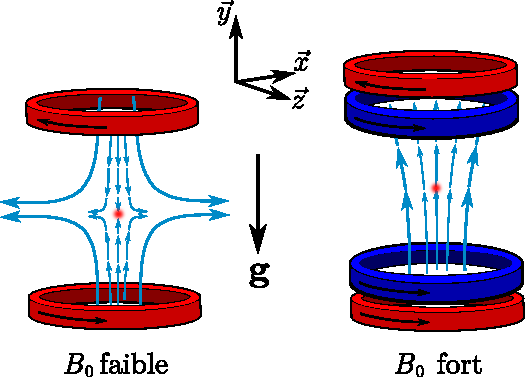
\includegraphics[scale=1]{Fig/BEC_manip/levitation_simple.pdf}
\caption{\textbf{Design simplifié de la lévitation magnétique}. Un gradient magnétique est appliqué aux atomes grâce à une paire de bobines parcourues par des courants opposés. La conservation du flux magnétique entraîne des gradients dans les autres directions de l'espace. L'application d'un fort champ de biais créé par d'autres bobines permet de minimiser l'impact de ces gradients et de diminuer les fréquences de piégeage (ou d'anti-piégeage) associées.}
\label{fig:levitation_simple}
\end{figure}

Pour finir, citons un dernier avantage offert par la lévitation magnétique: la compensation de la gravité n'entraîne pas d'effet \emph{SAG}, c'est à dire que la gravité ne vient pas "pencher" le potentiel de notre piège optique. Nous avons donc la possibilité de pousser l'évaporation optique jusque dans un domaine où la gravité aurait normalement dû tirer les atomes en dehors du piège, nous pouvons ainsi évaporer beaucoup plus loin et atteindre des températures extrêmement basses.



\paragraph*{Refroidir encore plus}
L'assimilation d'un condensat de Bose-Einstein à une onde de matière monochomatique $\left| k=0 \right\rangle$ nécessite de pouvoir négliger la largeur de distribution de vitesses $\Delta k$, et implique donc d'obtenir des nuages extrêmement froids. Bien que la lévitation magnétique nous permette d'obtenir des températures particulièrement basses, le refroidissement peut être poussé encore plus loin. 

Une première technique consiste en une décompression du nuage à l'aide de l'ouverture adiabatique du piège. Cette décompression se traduit par une diminution des fréquences de piégeage, que l'on obtient en changeant la taille des faisceaux de piégeage. En pratique, il nous suffit de reculer le plan de focalisation de la pince de 4.5mm en une seconde à l'aide de la platine de translation comme illustré figure \ref{fig:delta_kick}. La température obtenue est alors donnée par le théorème d'équipartition de l'énergie:
\begin{equation}
T'=\frac{\omega_{\mathrm{r}}'}{\omega_{\mathrm{r}}}T
\end{equation}
avec $\omega_{\mathrm{r}}$ la fréquence de piégeage de la pince dans la direction radiale. L'abaissement de la température est donc obtenu par diminution de la densité du nuage, c'est à dire par dilution. Cette étape se déroule en même temps que l'évaporation optique.

À la fin du cycle d'évaporation et d'ouverture adiabatique, il reste environ $2 \times 10^5$ atomes dont environ 50\% forment un condensat de Bose-Einstein. Le potentiel chimique de la partie condensée est estimée à $\mu/h=40$Hz, et la température de la fraction thermique est d'environ 5nK. 

\begin{figure}
\centering
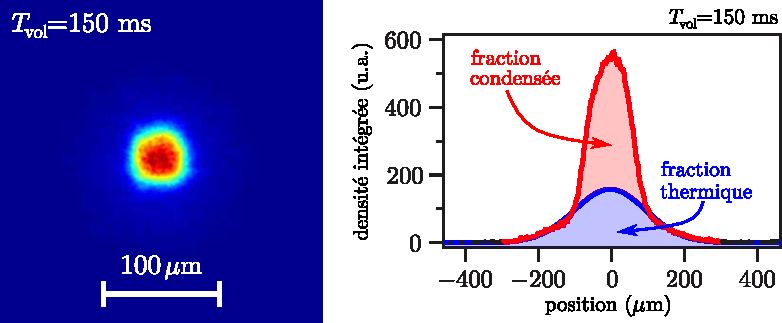
\includegraphics[width=0.9\textwidth]{Fig/BEC_manip/BEC_double_struct.pdf}
\caption{\textbf{Image expérimentale d'un condensat de Bose-Einstein}. Cette image correspond à celle d'un condensat après expansion pendant un temps de vol de 150ms. L'image de droite correspond au profil de la densité intégrée suivant une direction, et montre la double structure témoingnant d'une partie condensée. La partie condensée a un profil parabolique (en rouge), tandis que la partie thermique est de forme gaussienne (en bleu).}
\label{fig:BEC_double_struct}
\end{figure}


Après extinction du piège, l'énergie d'interaction de la partie condensée est convertie en énergie cinétique. 

Une dernière technique reposant aussi sur le principe de la dilution existe
delta-kick cooling: on cherche à affiner la distribution de vitesses. Pour cela on éteint le piège, et l'énergie d'interaction du condensat se transforme en énergie cinétique. Une fois suffisamment dilué, on applique un kick de potentiel pour figer la vitesse des atomes. 
En supposant que l'expansion des atomes est ballistique, la position des atomes après un temps d'expansion $t_{\mathrm{exp}}$ suffisamment grand est donnée par leur vitesse initiale:
\begin{equation}
\mathbf{r}(t_{\mathrm{exp}})=\mathbf{v} t_{\mathrm{exp}}
\end{equation}
Et appliquons un kick de potentiel pendant un temps $\Delta t$. La vitesse des atomes à la fin de ce kick est donnée par
\begin{equation}
\dot{\mathbf{r}}(\Delta t) = -\mathbf{r} \omega \sin{(\omega \Delta t)}+ \mathbf{v} \cos{(\omega \Delta t)}
\end{equation}
avec $\omega$ la fréquence du piège.
On peut trouver $\Delta t$ tel que $\dot{\mathbf{r}}_i=0$:
\begin{equation}
\Delta t= \frac{1}{\omega} \arctan{(\frac{1}{t_{\mathrm{exp}} \omega})}
\end{equation}
On remarque que $\Delta t$ ne dépend pas de la vitesse initiale des atomes: on peut donc geler l'ensemble du nuage. 
La mise en œuvre expérimentale de cette technique est détaillée dans le manuscrit de thèse de Kilian Muller \citep{muller2015coherent} et témoigne de résultats impressionnants: 

\begin{figure}
\centering
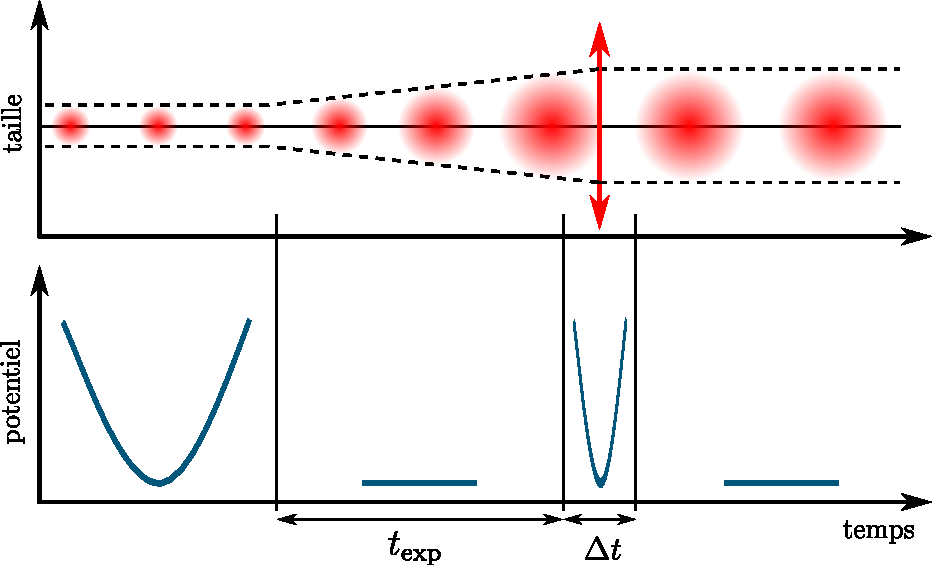
\includegraphics[width=0.8\textwidth]{Fig/BEC_manip/delta_kick.pdf}
\caption{delta kick cooling}
\label{fig:delta_kick}
\end{figure}















\subsection{Imagerie}
À la fin de la majorité de nos cycles expérimentaux, nous souhaitons obtenir des informations à propos de notre gaz d'atomes. Une grande partie de ces informations peut être extraite d'une image du nuage après extinction du piège, image que l'on obtient à l'aide d'une caméra et l'utilisation de lasers à résonance avec les atomes \footnote{L'utilisation de lasers à résonance conduit inévitablement à la destruction du nuage sur notre expérience. Il est donc nécessaire de répéter l'ensemble du cycle expérimental pour obtenir une seconde image des atomes.}. L'utilisation d'un retard (appelé \emph{temps de vol} et abrégé en \emph{TOF} pour l'anglais \textit{Time Of Flight}) entre l'extinction du piège et la prise de l'image est extrêmement courant fournit de précieux renseignements.

\paragraph*{Dispositif d'imagerie}
L'expérience est équipée de trois caméras \textit{EMCCD C9102} de chez \textit{Hamamatsu}, chacune comportant une matrice de $1000 \times 1000$ pixels de taille 8µm $\times$ 8µm. Ces trois caméras sont contrôlées via l'outil d'acquisition d'images de MATLAB, qui permet aussi de récupérer et traiter les images obtenues. L'acquisition des images est déclenchée de manière externe par le séquenceur.\\
Une première caméra acquiert des images des atomes dans la première chambre selon l'axe horizontal $\vec{x}$ avec un grandissement de 1, la zone imageable est donc de 8mm $\times$ 8mm. Il est possible d'utiliser cette caméra pour de l'imagerie par absorption (représentée figure \ref{fig:img_mot}) aussi que pour de l'imagerie par fluoresence grâce à un montage 4$f$. Néanmoins, l'observation selon une direction induit forcément une intégration de la densité suivant cette direction: on ne peut mesurer qu'une densité intégrée.
\begin{equation}
n_{\mathrm{2D}}(y,z) =\int{\mathrm{d}x \: n(x,y,z)}
\end{equation}
avec $n$ la densité à trois dimensions.\\
Les deux autres caméras sont positionnées autour de la chambre de science selon l'axe horizontal $\vec{x}$ et vertical $\vec{y}$. Toutes deux voient le nuage au travers d'un système optique de grandissement 3\footnote{Ce grandissement a été mesuré on observant la chute libre du nuage en l'absence de la lévitation.}, conduisant à une résolution de 2.71µm pour une zone imageable de 2.71mm $\times$ 2.71mm. Seule de l'imagerie par fluorescence est utilisable dans cette chambre, en revanche il est possible d'utiliser ces deux caméras simultanément pour obtenir les densités intégrés suivant deux directions $n_{\mathrm{2D}}(y,z)$ et $n_{\mathrm{2D}}(x,y)$ pour le même nuage.

\paragraph*{Imagerie par absorption}
Le principe de l'imagerie par absorption repose sur la loi de Beer-Lambert. En effet, lorsque qu'un faisceau laser traverse un milieu, son absorption dépend directement de la densité du milieu en particules absorbantes (la densité atomique dans notre cas). Pour sonder cette densité atomique, on envoie donc un faisceau laser à résonance directement sur les atomes et la caméra comme illustré figure \ref{fig:img_mot}. 
\begin{figure}
\centering
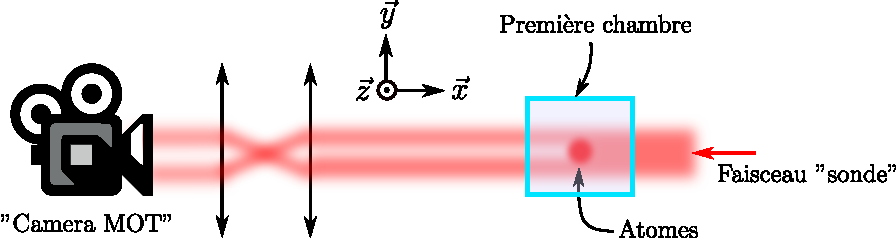
\includegraphics[width=\textwidth]{fig/BEC_manip/img_mot.pdf}
\caption{\textbf{Imagerie par absorption.} Un faisceau collimaté est envoyé sur les atomes, qui absorbent une partie des photons qui traversent le nuage. Le signal détecté à la caméra correspond à "l'ombre" des atomes, et la comparaison avec une image du faisceau incident sans atomes permet de remonter à la densité atomique intégrée selon la direction longitudinale.}
\label{fig:img_mot}
\end{figure}
Dans un régime de très basse saturation $s \ll 1$, on peut montrer que la section efficace d'absorption de photons $\sigma$ est indépendante de l'intensité incidente $I_0(y,z)$. En pratique, on garde la puissance du faisceau \emph{sonde} en dessous de 100µW pour s'en assurer. Le faisceau \emph{sonde} correspond à une impulsion lumineuse d'une durée de 50µs réalisée par un laser à résonance avec la transition $\left| F=2 \right\rangle \rightarrow \left| F'=3 \right\rangle$ et permet ainsi de mesurer la densité atomique dans l'état $\left| F=2 \right\rangle$. \\
Afin de mesurer aussi les atomes qui sont dans l'état $\left| F=1 \right\rangle$, on procède à un transfert de population vers l'état $\left| F=2 \right\rangle$ à l'aide d'une impulsion du faisceau repompeur accordé sur la transition $\left| F=1 \right\rangle \rightarrow \left| F'=2 \right\rangle$ pendant une durée de 40µs . Ce transfert est réalisé à la fin du temps de vol, juste avant le déclenchement de la caméra. \\
L'application de la loi de Beer-Lambert permet de déterminer la densité atomique intégrée suivant l'axe longitudinal:
\begin{equation}
n_{\mathrm{2D}}(y,z)= \frac{1}{\sigma} \mathrm{ln}\left( \frac{I_0(y,z)}{I(y,z)} \right)
\end{equation}
L'opération de reconstruction du profil de densité atomique nécessite donc deux images: une image des atomes absorbant une partie du faisceau \emph{sonde}, et une image de ce faisceau sans les atomes pour connaître le profil d'intensité $I_0(y,z)$. En pratique, on prend une troisième image afin de soustraire le bruit de fond. De plus, une bonne reconstruction du profil nécessite des contraintes supplémentaires. En effet, nous nous fixons de travailler dans un régime où la sonde ne sature pas la caméra (cela fixe une borne supérieure pour l'intensité du faisceau), et où l'absorption de photons n'est pas totale dans les régions les plus denses.



\paragraph*{Imagerie par fluorescence}
Le principe de l'imagerie par fluorescence consiste à éclairer les atomes avec de la lumière à résonance, puis à détecter la lumière que les atomes diffusent comme illustré figure \ref{fig:img_science}. Pour cela, on envoie des faisceaux très saturants $s \gg 1$ sur les atomes afin que le taux d'émission spontanée ne dépende plus de l'intensité incidente. Un avantage de cette technique par rapport à l'imagerie par absorption est sa capacité à détecter de très faibles nombres d'atomes, rendu possible grâce à l'amplification des caméras. Un deuxième avantage réside dans la simplicité de sa mise en œuvre: l'imagerie dans la première chambre est réalisée à l'aide des faisceaux MOT. L'imagerie de la seconde chambre est quant à elle réalisée à l'aide de deux autres faisceaux dédiés.
\begin{figure}
\centering
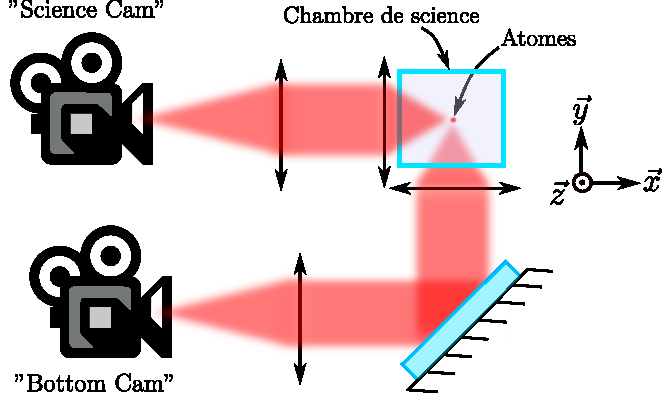
\includegraphics[scale=1]{fig/BEC_manip/img_science_3.pdf}
\caption{\textbf{Dispositif d'imagerie par fluorescence pour la chambre de science.} Une caméra capte les photons de fluorescence émis par les atomes selon une direction horizontale (\emph{Science Cam}), tandis qu'une autre capte ceux émis vers le bas avec un transport d'image (\emph{Bottom Cam}). Les faisceaux de fluorescence ne sont pas représentés ici (selon l'axe $\vec{z}$).}
\label{fig:img_science}
\end{figure}
Les faisceaux d'imagerie sont à résonance avec la transition $\left| F=2 \right\rangle \rightarrow \left| F'=3 \right\rangle$ et permettent donc de sonder les atomes se trouvant dans l'état $\left| F=2 \right\rangle$. Comme pour l'imagerie par absorption, il est aussi possible d'adresser les atomes qui sont dans l'état $\left| F=1 \right\rangle$. Pour cela, on superpose aux faisceaux de fluorescence le faisceau repompeur\footnote{Les faisceaux de refroidissement laser et de fluorescence comportent déjà une partie de repompeur: le mélange se fait avant les amplificateurs optiques et il est possible de couper la partie repompeur à l'aide d'un obturateur mécanique, voir figure \ref{fig:table_optique}.}, accordé sur $\left| F=1 \right\rangle \rightarrow \left| F'=2 \right\rangle$ pendant toute la durée de l'impulsion lumineuse, qui est typiquement de 50µs. \\
L'intensité fluorescée captée dans le plan d'imagerie est alors donnée par:
\begin{equation}
I_{\mathrm{fluo}}(y,z)=\frac{\Omega}{4\pi} \frac{s}{1+s} \frac{ \Gamma \hb \omega_0}{2} n_{\mathrm{2D}}(y,z)
\label{eq:img_fluo}
\end{equation}
avec $\Omega \simeq \pi \mathrm{ON}^2$ l'angle solide dans lequel les photons de fluorescence sont captés par le système d'imagerie d'ouverture numérique $\mathrm{ON}\sim 0.4$. \\
Théoriquement, une seule image suffit à obtenir le profil de densité atomique. Cependant, on décide de prendre une seconde image avec les faisceaux de fluorescence allumés afin de soustraire un éventuel bruit dû à ces faisceaux. Pour des raisons de simplicité de configuration des caméras, on décide aussi de prendre une troisième image du bruit de fond, non utilisée pour le calcul de densité atomique.\\
Étant donné le nombre de paramètres non parfaitement connus dans la formule \ref{eq:img_fluo}, il est nécessaire de calibrer cette méthode d'imagerie. La calibration du nombre d'atomes se fait par comparaison avec l'imagerie par absorption. Si la comparaison est directe dans la première chambre, celle de l'imagerie dans la chambre de science est un peu plus délicate. La méthode retenue par l'équipe consiste à calibrer l'efficacité du transfert par la pince optique à l'aide d'allers-retours pour déterminer le nombre d'atomes attendu dans la seconde chambre.


